\documentclass[11pt]{article}
\usepackage[margin=.72in]{geometry}
\usepackage{amsmath,amssymb,lmodern,microtype,tikz,tcolorbox,fancyhdr,xcolor}
\usetikzlibrary{arrows.meta,patterns}
\tcbuselibrary{breakable}
\definecolor{navy}{RGB}{27,57,95}\definecolor{blue}{RGB}{47,117,181}\definecolor{amber}{RGB}{178,91,0}
\setlength{\parindent}{0pt}\setlength{\parskip}{9pt}\setlength{\jot}{14pt}\allowdisplaybreaks[1]
\pagestyle{fancy}\fancyhf{}\fancyhead[L]{Electricity \& Magnetism I}\fancyhead[R]{Lesson 14}\fancyfoot[C]{\thepage}\setlength{\headheight}{15pt}
\newcommand{\heading}[2]{\begin{center}{\LARGE\bfseries\color{navy} #1}\\[5pt]{\large #2}\end{center}\vspace{2pt}\hrule\vspace{9pt}}
\newcommand{\topic}[1]{\par{\Large\bfseries\color{navy}#1}\par}
\newcommand{\q}[2]{\par\bigskip\noindent\textbf{\color{navy}#1}\par\smallskip #2\par\medskip}
\newcommand{\work}[1]{\par\begin{center}\begin{tikzpicture}\draw[gray!45] (0,0) rectangle (15.3,{0.72*#1});\end{tikzpicture}\end{center}}
\newcommand{\concept}[2]{\begin{tcolorbox}[colback=blue!7,colframe=blue,title=#1,fonttitle=\bfseries,boxrule=.6pt,breakable]#2\end{tcolorbox}}
\newcommand{\coach}[1]{\begin{tcolorbox}[colback=blue!3,colframe=blue!55,title=Guided starting point,fonttitle=\bfseries,boxrule=.5pt,breakable]#1\end{tcolorbox}}
\newcommand{\route}[1]{\begin{tcolorbox}[colback=yellow!5,colframe=amber,title=Where this fits,fonttitle=\bfseries,boxrule=.5pt,breakable]#1\end{tcolorbox}}
\newcommand{\pausecheck}[1]{\begin{tcolorbox}[colback=white,colframe=navy!65,title=Check your thinking,fonttitle=\bfseries,boxrule=.5pt,breakable]#1\end{tcolorbox}}
\newcommand{\bridge}[1]{\begin{tcolorbox}[colback=white,colframe=amber,title=Physical starting point,fonttitle=\bfseries,boxrule=.5pt,breakable]#1\end{tcolorbox}}
\newcommand{\stage}[1]{\par\medskip\noindent\textbf{\color{blue}#1}\par\smallskip}
\newcommand{\connect}[1]{\begin{tcolorbox}[colback=blue!4,colframe=blue!45,title=Keep the thread,fonttitle=\bfseries,boxrule=.45pt,breakable]#1\end{tcolorbox}}


\newcommand{\dipfig}{\begin{center}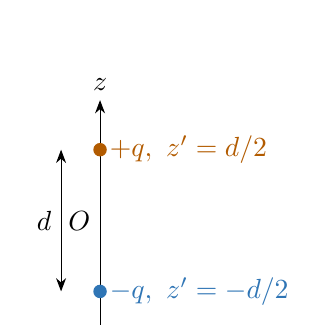
\begin{tikzpicture}[>=Stealth,scale=.9]
\draw[->] (0,-1.65)--(0,1.7) node[above] {$z$};
\fill[amber] (0,1) circle (.095) node[right] {$+q,\ z'=d/2$};
\fill[blue] (0,-1) circle (.095) node[right] {$-q,\ z'=-d/2$};
\node[left] at (0,0) {$O$};\draw[<->] (-.55,-1)--(-.55,1) node[midway,left] {$d$};
\end{tikzpicture}\end{center}}
\newcommand{\ringfig}{\begin{center}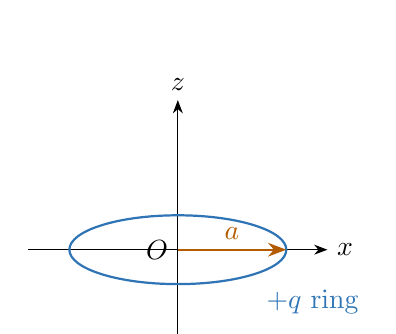
\begin{tikzpicture}[>=Stealth,scale=.95]
\draw[->] (0,-1.3)--(0,2) node[above] {$z$};
\draw[->] (-2,0)--(2,0) node[right] {$x$};
\draw[blue,thick] (0,0) ellipse (1.45 and .46);
\draw[->,amber,thick] (0,0)--(1.45,0) node[midway,above] {$a$};
\node[blue] at (1.8,-.7) {$+q$ ring};\node[left] at (0,0) {$O$};
\end{tikzpicture}\end{center}}
\newcommand{\linefig}{\begin{center}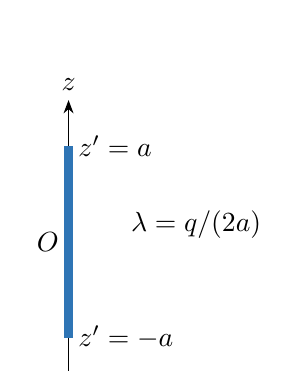
\begin{tikzpicture}[>=Stealth,scale=.9]
\draw[->] (0,-2)--(0,2) node[above] {$z$};
\draw[blue,line width=3pt] (0,-1.35)--(0,1.35);
\node[right] at (0,1.35) {$z'=a$};\node[right] at (0,-1.35) {$z'=-a$};
\node[left] at (0,0) {$O$};\node at (1.8,.25) {$\lambda=q/(2a)$};
\end{tikzpicture}\end{center}}
\begin{document}
\heading{Multipole Expansion: Five Charge Distributions}{Comprehensive Worked Answer Key — Revised for Mathematical Clarity}
\concept{Problem-solving thread}{Each activity follows the same route: identify the source, locate $R_{\max}$, choose and normalize $dQ$, evaluate $Q_n$, apply symmetry, and interpret the exterior potential. The mathematical explanations below accompany every question.}
\concept{Convention}{The guide uses $\theta$ for polar angle and $\phi$ for azimuth, opposite the student's preferred naming. All expressions retain the lecture convention.}
\topic{Activity 1: Choose the correct multipole setup}
\bridge{Every example begins with source geometry, the charge element, and the convergence region. The index $n$ labels angular patterns, not individual charges.}

\q{1a.}{Explain the meaning of $r$, $r^\prime$, $\theta^\prime$, $dQ$, $Q_n$, and $R_{\max}$. Write the moment formula and the first three terms of the potential.}
\stage{Physical setup and step-by-step solution}

\stage{Identify what moves and what stays fixed}
The observation point $(r,\theta)$ is fixed while we sum over the source positions $(r',\theta',\phi')$. A source element carries actual charge $dQ$; the moment $Q_n$ weights that charge by its position and angular pattern.
\stage{Write the moment before the potential}
\[\boxed{Q_n=\int_{\rm source}r'^nP_n(\cos\theta')\,dQ.}\]
\stage{Insert one moment at a time}
\begin{align*}V(r,\theta)&=\frac1{4\pi\epsilon_0}\sum_{n=0}^\infty\frac{Q_n}{r^{n+1}}P_n(\cos\theta)\\&=\frac1{4\pi\epsilon_0}\left[\frac{Q_0}{r}+\frac{Q_1}{r^2}P_1(\cos\theta)+\frac{Q_2}{r^3}P_2(\cos\theta)+\cdots\right].\end{align*}
\stage{State the domain}
This exterior expansion requires $r>R_{\max}$, where $R_{\max}$ is the greatest source distance from the chosen origin.
\connect{Distinguish a small piece of physical charge $dQ$ from its weighted moment $Q_n$.}

\q{1b.}{Match each source to its charge element: point charges, a line, a ring, and a spherical cloud. Explain how to check normalization.}
\stage{Physical setup and reasoning}

For points, $Q_n=\sum_i q_i r_i^{\prime n}P_n(\cos\theta_i^\prime)$. For a line, $dQ=\lambda\,d\ell^\prime$; for a ring, $dQ=\lambda a\,d\phi^\prime$; for a cloud, $dQ=\rho r^{\prime2}\sin\theta^\prime dr^\prime d\theta^\prime d\phi^\prime$. Always integrate $dQ$ alone first: $\int dQ=q_{\rm total}=Q_0$.
\connect{For a ring $d\ell^\prime=a\,d\phi^\prime$; for a cloud $d\tau^\prime=r^{\prime2}\sin\theta^\prime dr^\prime d\theta^\prime d\phi^\prime$.}

\q{1c.}{Predict which moments vanish for a distribution unchanged under $z\mapsto-z$, and for one whose signed charge reverses under that reflection. Justify using $P_n(-x)=(-1)^nP_n(x)$.}
\stage{Physical setup and reasoning}

For a reflection-even distribution, paired contributions are proportional to $P_n(x)+P_n(-x)=[1+(-1)^n]P_n(x)$, zero for odd $n$. For a reflection-odd signed distribution, contributions are proportional to $P_n(x)-P_n(-x)=[1-(-1)^n]P_n(x)$, zero for even $n$.
\connect{Pair source elements at opposite $z$ with the same $r^\prime$.}

\newpage
\topic{Activity 2: A single point charge at the origin}
\bridge{Begin with the simplest source. This example also reveals why the multipole moments depend on the chosen origin.}

\q{2a.}{For a point charge $+q$ at the origin, identify $R_{\max}$ and evaluate $Q_0$ without a volume integral.}
\stage{Physical setup and reasoning}

All source charge is at $r^\prime=0$, so $R_{\max}=0$. The monopole is $Q_0=q(r^\prime)^0P_0=q$. The origin has no preferred direction.
\connect{Use the discrete-charge sum and $P_0=1$.}

\q{2b.}{Explain why every $Q_n$ with $n\ge1$ vanishes, even though the polar angle at the origin is undefined.}
\stage{Physical setup and reasoning}

Because $|P_n(\cos\theta^\prime)|\le1$, $|r^{\prime n}P_n|\le r^{\prime n}\to0$ as $r^\prime\to0$ for $n\ge1$. Thus $Q_n=0$ for every higher moment, independent of the undefined direction at the origin.
\connect{The factor $r^{\prime n}P_n(\cos\theta^\prime)$ tends to zero as $r^\prime\to0$ for $n\ge1$.}

\q{2c.}{Write the complete exterior potential and check its angular dependence and domain. What changes if the coordinate origin moves?}
\stage{Physical setup and reasoning}


\[\boxed{V(r)=\frac{q}{4\pi\epsilon_0r}},\qquad r>0.\]
 It is angle-independent, as spherical symmetry demands. If the origin is moved, the charge acquires nonzero source radius $r^\prime$ and generally higher moments about that new origin.
\connect{Only $Q_0$ survives for the centered charge.}

\newpage
\topic{Activity 3: Two opposite charges on the polar axis}
\bridge{For the axial dipole, the charge signs and position signs both matter. Calculate the first moments explicitly before generalizing.}

\q{3a.}{Draw $+q$ at $z=d/2$ and $-q$ at $z=-d/2$. Label their radii and polar angles, then determine $R_{\max}$.}
\stage{Physical setup and reasoning}

\dipfig Both charges have $r^\prime=d/2$. The upper charge has $\theta^\prime=0$; the lower has $\theta^\prime=\pi$. Hence $R_{\max}=d/2$.
\connect{Both source radii equal $d/2$, but their polar angles are $0$ and $\pi$.}

\q{3b.}{Calculate $Q_0$, $Q_1$, $Q_2$, and $Q_3$ separately, showing the contribution from each charge. Explain the parity pattern.}
\stage{Physical setup and step-by-step solution}

\stage{Write the two source contributions separately}
The upper source has charge $+q$, radius $d/2$, and $\cos\theta'=1$. The lower source has charge $-q$, the same radius, and $\cos\theta'=-1$.
\begin{align*}Q_n&=(+q)\left(\frac d2\right)^nP_n(1)+(-q)\left(\frac d2\right)^nP_n(-1)\\&=q\left(\frac d2\right)^n\left[P_n(1)-P_n(-1)\right]\\&=q\left(\frac d2\right)^n\left[1-(-1)^n\right].\end{align*}
\stage{Monopole: $n=0$}
\begin{align*}Q_0&=q-q\\&=0.\end{align*}
\stage{Dipole: $n=1$}
\begin{align*}Q_1&=(+q)\frac d2+(-q)\left(-\frac d2\right)\\&=\frac{qd}{2}+\frac{qd}{2}\\&=qd.\end{align*}
\stage{Quadrupole: $n=2$}
\begin{align*}Q_2&=q\frac{d^2}{4}-q\frac{d^2}{4}\\&=0.\end{align*}
\stage{Octupole: $n=3$}
\begin{align*}Q_3&=q\left(\frac d2\right)^3\left[1-(-1)^3\right]\\&=2q\frac{d^3}{8}\\&=\frac{qd^3}{4}.\end{align*}
The source reverses sign under $z\mapsto-z$, so all even moments vanish.
\connect{Use $P_n(1)=1$ and $P_n(-1)=(-1)^n$.}

\q{3c.}{Write the first two nonzero potential terms. Identify the leading far-field term and explain its direction.}
\stage{Physical setup and reasoning}


\[V(r,\theta)=\frac1{4\pi\epsilon_0}\left[\frac{qd\cos\theta}{r^2}+\frac{qd^3P_3(\cos\theta)}{4r^4}+\cdots\right],\quad r>d/2.\]
 For $r\gg d$, the dipole term dominates: $V\simeq qd\cos\theta/(4\pi\epsilon_0r^2)$. The dipole moment is $qd\,\hat{\mathbf z}$.
\connect{The dipole moment points from the negative charge to the positive charge.}

\newpage
\topic{Activity 4: A spherical charge cloud}
\bridge{The density $f(r^\prime)$ can vary radially. Spherical symmetry, not uniform density, removes the higher exterior moments.}

\q{4a.}{For $\rho=f(r^\prime)$ inside $r^\prime\le a$, write $dQ$, the integration limits, and the normalization equation for total charge $q$.}
\stage{Physical setup and reasoning}


\[dQ=f(r^\prime)r^{\prime2}\sin\theta^\prime\,dr^\prime d\theta^\prime d\phi^\prime.\]
 Limits: $0\le r^\prime\le a$, $0\le\theta^\prime\le\pi$, $0\le\phi^\prime<2\pi$. Integrating charge: 
\[q=\int_0^a f(r^\prime)r^{\prime2}dr^\prime\int_0^\pi\sin\theta^\prime d\theta^\prime\int_0^{2\pi}d\phi^\prime=4\pi\int_0^a f(r^\prime)r^{\prime2}dr^\prime.\]

\connect{The volume element contains $r^{\prime2}\sin\theta^\prime$.}

\q{4b.}{Factor the moment integral into radial and angular pieces. With $u=\cos\theta^\prime$, show why $Q_n=0$ for $n\ge1$.}
\stage{Physical setup and step-by-step solution}

\stage{Start from the correct volume charge element}
\[dQ=f(r')r'^2\sin\theta'\,dr'\,d\theta'\,d\phi'.\]
\stage{Insert it into the moment definition}
\[Q_n=\int_0^a\!\int_0^\pi\!\int_0^{2\pi}r'^nP_n(\cos\theta')f(r')r'^2\sin\theta'\,d\phi'\,d\theta'\,dr'.\]
\stage{Separate independent variables}
\[Q_n=\left[\int_0^af(r')r'^{n+2}dr'\right]\left[\int_0^\pi P_n(\cos\theta')\sin\theta'\,d\theta'\right]\left[\int_0^{2\pi}d\phi'\right].\]
The last integral equals $2\pi$.
\stage{Change the polar integration variable}
Let $u=\cos\theta'$, so $du=-\sin\theta'\,d\theta'$. The original limits $0,\pi$ become $1,-1$:
\begin{align*}\int_0^\pi P_n(\cos\theta')\sin\theta'\,d\theta'&=-\int_1^{-1}P_n(u)\,du\\&=\int_{-1}^1P_n(u)\,du\\&=2\delta_{n0}.\end{align*}
The final equality uses orthogonality with $P_0(u)=1$.
\stage{Interpret the cancellation}
Thus $Q_n=0$ for $n\ge1$, while
\[Q_0=4\pi\int_0^af(r')r'^2\,dr'=q.\]
No uniform-density assumption was needed.
\connect{Show the transformed limits $\theta^\prime=0\to u=1$ and $\theta^\prime=\pi\to u=-1$.}

\q{4c.}{Give the exterior potential and explain why the same expression is not automatically valid inside the cloud.}
\stage{Physical setup and reasoning}


\[\boxed{V(r)=\frac{q}{4\pi\epsilon_0r}},\quad r>a.\]
 Spherical symmetry makes the exterior potential identical to that of a point charge at the origin. Inside, the enclosed charge varies with radius and the potential depends on $f(r^\prime)$; the exterior expression cannot be extended inward without solving that region.
\connect{The exterior series requires $r>a$; interior charge contributes differently.}

\newpage
\topic{Activity 5: A uniformly charged circular ring}
\bridge{All ring elements have the same radius and polar angle. Geometry makes the moment integral simple; the angular sign is important.}

\q{5a.}{Sketch the ring in the $xy$ plane. Label its radius $a$, polar angle $\theta^\prime$, line density $\lambda$, and charge element $dQ$. Verify the total charge.}
\stage{Physical setup and reasoning}

\ringfig Each source element has $r^\prime=a$ and $\theta^\prime=\pi/2$. The line density is $\lambda=q/(2\pi a)$, so $dQ=\lambda a\,d\phi^\prime=q\,d\phi^\prime/(2\pi)$. Integrating from $0$ to $2\pi$ gives total charge $q$.
\connect{Use $\theta^\prime=\pi/2$, $d\ell^\prime=a\,d\phi^\prime$, and $\lambda=q/(2\pi a)$.}

\q{5b.}{Derive $Q_n=qa^nP_n(0)$. Compute $Q_0$, $Q_2$, and $Q_4$ and explain why odd moments vanish.}
\stage{Physical setup and step-by-step solution}

\stage{Use the ring geometry before integrating}
Every source element has $r'=a$ and $\cos\theta'=0$. The charge element is
\[dQ=\frac{q}{2\pi}\,d\phi'.\]
\stage{Evaluate the angular integral}
\begin{align*}Q_n&=\int_0^{2\pi}a^nP_n(0)\frac{q}{2\pi}\,d\phi'\\&=\frac{qa^nP_n(0)}{2\pi}\left[\phi'\right]_0^{2\pi}\\&=qa^nP_n(0).\end{align*}
\stage{Evaluate the first three even modes}
\begin{align*}Q_0&=qP_0(0)=q,\\Q_2&=qa^2P_2(0)=-\frac{qa^2}{2},\\Q_4&=qa^4P_4(0)=\frac{3qa^4}{8}.\end{align*}
\stage{Explain the missing odd modes}
For odd $n$, $P_n(0)=0$, so $Q_n=0$. The negative $Q_2$ reflects the equatorial geometry, not negative charge.
\connect{Use $P_2(0)=-1/2$ and $P_4(0)=3/8$.}

\q{5c.}{Write the first three nonzero terms of $V(r,\theta)$. Check the axis result against the exact ring potential $V(r,0)=q/(4\pi\epsilon_0\sqrt{r^2+a^2})$.}
\stage{Physical setup and reasoning}


\[V=\frac{q}{4\pi\epsilon_0r}\left[1-\frac12\left(\frac ar\right)^2P_2(\cos\theta)+\frac38\left(\frac ar\right)^4P_4(\cos\theta)+\cdots\right],\quad r>a.\]
 On the axis $P_2(1)=P_4(1)=1$, giving $1-a^2/(2r^2)+3a^4/(8r^4)+\cdots$. Independently, $1/\sqrt{r^2+a^2}=r^{-1}(1+a^2/r^2)^{-1/2}$ has the same binomial expansion.
\connect{Factor out $1/r$ and expand $(1+a^2/r^2)^{-1/2}$.}

\newpage
\topic{Activity 6: A finite uniformly charged axial line}
\bridge{Unlike the ring, the line lies on the polar axis. Its quadrupole has the opposite sign even though both carry positive charge.}

\q{6a.}{Sketch the line from $z=-a$ to $z=a$. Find $\lambda$, $R_{\max}$, and the two polar angles needed to split the integral.}
\stage{Physical setup and reasoning}

\linefig The total length is $2a$, so $\lambda=q/(2a)$ and $R_{\max}=a$. For the upper half $P_n(\cos\theta^\prime)=P_n(1)=1$; for the lower half $P_n(-1)=(-1)^n$.
\connect{Upper half: $\theta^\prime=0$; lower half: $\theta^\prime=\pi$.}

\q{6b.}{Split the moment into upper and lower integrals over $0\le r^\prime\le a$. Integrate and obtain the general even/odd result.}
\stage{Physical setup and step-by-step solution}

\stage{Separate the upper and lower halves}
The upper half has polar angle $0$ and the lower half has polar angle $\pi$. Each half extends from source radius $r'=0$ to $r'=a$.
\[Q_n=\lambda\int_0^a r'^nP_n(1)\,dr'+\lambda\int_0^a r'^nP_n(-1)\,dr'.\]
\stage{Use endpoint values of Legendre polynomials}
\begin{align*}Q_n&=\lambda\int_0^ar'^n\,dr'+\lambda(-1)^n\int_0^ar'^n\,dr'\\&=\lambda\left[1+(-1)^n\right]\int_0^ar'^n\,dr'.\end{align*}
\stage{Perform the power-law integral}
\begin{align*}\int_0^ar'^n\,dr'&=\left[\frac{r'^{n+1}}{n+1}\right]_0^a\\&=\frac{a^{n+1}}{n+1}.\end{align*}
Therefore
\[Q_n=\frac{\lambda a^{n+1}}{n+1}\left[1+(-1)^n\right].\]
\stage{Substitute the normalized line density}
With $\lambda=q/(2a)$,
\begin{align*}Q_n&=\frac{qa^n}{2(n+1)}\left[1+(-1)^n\right]\\&=\begin{cases}\dfrac{qa^n}{n+1},&n\text{ even},\\[5pt]0,&n\text{ odd}.\end{cases}\end{align*}
The odd modes cancel between opposite halves of the same positively charged line.
\connect{Use $\int_0^a r^{\prime n}dr^\prime=a^{n+1}/(n+1)$.}

\q{6c.}{Find $Q_0$, $Q_2$, and $Q_4$, write the exterior series through $n=4$, and compare the sign of $Q_2$ with the ring.}
\stage{Physical setup and reasoning}

$Q_0=q$, $Q_2=qa^2/3$, and $Q_4=qa^4/5$. Therefore 
\[V=\frac{q}{4\pi\epsilon_0r}\left[1+\frac13\left(\frac ar\right)^2P_2(\cos\theta)+\frac15\left(\frac ar\right)^4P_4(\cos\theta)+\cdots\right],\quad r>a.\]
 The line quadrupole is positive because $P_2(\pm1)=1$; the ring quadrupole is negative because $P_2(0)=-1/2$.
\connect{On the polar axis $P_2(\pm1)=1$, whereas the ring has $P_2(0)=-1/2$.}

\newpage
\topic{Activity 7: Compare, combine, and choose the leading term}
\bridge{Use symmetry and superposition to solve a new problem without starting the integration over again.}

\q{7a.}{Complete a comparison: for the five lesson sources, give $R_{\max}$, which moments survive, and the leading far-field potential.}
\stage{Physical setup and reasoning}

\begin{center}\small\begin{tabular}{lccc}Source&$R_{\max}$&Surviving modes&Leading $V$\\\hline Point at origin&$0$&$n=0$&$q/(4\pi\epsilon_0r)$\\ Axial $\pm q$&$d/2$&odd&$qd\cos\theta/(4\pi\epsilon_0r^2)$\\ Spherical cloud&$a$&$n=0$&$q/(4\pi\epsilon_0r)$\\ Ring&$a$&even&$q/(4\pi\epsilon_0r)$\\ Axial line&$a$&even&$q/(4\pi\epsilon_0r)$\end{tabular}\end{center}
\connect{For nonzero net charge, the monopole is leading even when higher moments are present.}

\q{7b.}{A concentric spherical cloud carries $+q$ and a uniformly charged ring of radius $a$ carries $-q$. Find $Q_0$ and $Q_2$ and the leading far-field potential.}
\stage{Physical setup and step-by-step solution}

\stage{Use linearity rather than reintegrating}
The spherical cloud contributes only its monopole:
\[Q_0^{\rm cloud}=+q,\qquad Q_2^{\rm cloud}=0.\]
The ring has charge $-q$, so its first moments are
\begin{align*}Q_0^{\rm ring}&=-q,\\Q_2^{\rm ring}&=(-q)a^2P_2(0)\\&=(-q)a^2\left(-\frac12\right)\\&=\frac{qa^2}{2}.\end{align*}
\stage{Add corresponding moments}
\begin{align*}Q_0^{\rm total}&=q-q=0,\\Q_1^{\rm total}&=0,\\Q_2^{\rm total}&=0+\frac{qa^2}{2}=\frac{qa^2}{2}.\end{align*}
The first nonzero mode is quadrupolar.
\stage{Insert it into the potential series}
\begin{align*}V(r,\theta)&\simeq\frac1{4\pi\epsilon_0}\frac{Q_2}{r^3}P_2(\cos\theta)\\&=\boxed{\frac{qa^2}{8\pi\epsilon_0r^3}P_2(\cos\theta)}.\end{align*}
This holds in the far field beyond both the ring and the cloud.
\connect{The cloud has only a monopole; the ring has $Q_2=q_{\rm ring}a^2P_2(0)$.}

\q{7c.}{For a generic source, state three checks that can catch an incorrect moment calculation: normalization, units, and convergence domain. Explain how each check works.}
\stage{Physical setup and reasoning}

Normalization: $Q_0=\int dQ$ must equal net charge. Units: each factor $r^{\prime n}$ gives $[Q_n]=\mathrm{C\,m}^n$, so $Q_n/r^{n+1}$ has units $\mathrm{C/m}$ and multiplication by $1/(4\pi\epsilon_0)$ gives volts. Domain: require $r>R_{\max}$ for every source point; merely being outside some portion of the material is insufficient.
\connect{$[Q_n]=\mathrm{C\,m}^n$ and the series needs $r>R_{\max}$.}
\end{document}